\RequirePackage{plautopatch}
\documentclass[dvipdfmx,uplatex,a4j,10pt,oneside]{jsarticle}
\usepackage{datetime}
\usepackage{float}
\usepackage{graphicx}
\usepackage{listings}
\usepackage{multicol}

% List
\usepackage{enumitem}
\renewcommand{\labelitemi}{$\bullet$}
\renewcommand{\labelitemii}{$\circ$}
\renewcommand{\labelitemiii}{$\bullet$}
\renewcommand{\labelitemiv}{$\circ$}

% Chapter Config
\renewcommand{\thesection}{\arabic{section}.}
\renewcommand{\thesubsection}{(\arabic{subsection})}
\renewcommand{\thesubsubsection}{\alph{subsubsection})}

% Figure and Table Name Config
\renewcommand{\figurename}{Fig.~}
\renewcommand{\tablename}{Table~}
\makeatletter
\def\fnum@table{{\bfseries{\sffamily\tablename\nobreak\thetable}}}
\def\fnum@figure{{\bfseries{\sffamily\figurename\nobreak\thefigure}}}
\makeatother
\newcommand{\refequation}[1]{式(\ref{#1})}
\newcommand{\reftable}[1]{{\bfseries{\sffamily{Table~\ref{#1}}}}}
\newcommand{\reffigure}[1]{{\bfseries{\sffamily{Fig.~\ref{#1}}}}}
\newcommand{\refcode}[1]{{\bfseries{\sffamily{Code~\ref{#1}}}}}

%% Font Config
\usepackage[deluxe]{otf}
\usepackage[noalphabet,unicode,haranoaji]{pxchfon}
\usepackage[prefernoncjk]{pxcjkcat}
\usepackage[utf8]{inputenc}
\usepackage[T1]{fontenc}
\usepackage{textcomp}
\usepackage{lmodern}
\usepackage{fix-cm}
\cjkcategory{sym18}{cjk}
\cjkcategory{sym19}{cjk}

%% Cites
\usepackage[autocite=superscript,maxnames=99,sorting=none]{biblatex}
\addbibresource{index.bib}
\renewcommand{\bibopenbracket}{}
\renewcommand{\bibclosebracket}{)}
\DeclareCiteCommand{\cite}[\mkbibsuperscript]
  {\iffieldundef{prenote}
     {}
     {\BibliographyWarning{Ignoring prenote argument}}%
   \iffieldundef{postnote}
     {}
     {\BibliographyWarning{Ignoring postnote argument}}%
   \bibopenbracket}%
  {\usebibmacro{citeindex}%
   \usebibmacro{cite}}
  {\supercitedelim}
  {\bibclosebracket}
\DeclareFieldFormat{url}{%
  \mkbibacro{URL}\addcolon\space
  \href{#1}{\nolinkurl{\thefield{urlraw}}}}
\AtBeginBibliography{\small}

%% Margin Config
\usepackage[top=19truemm,bottom=24truemm,left=20truemm,right=20truemm]{geometry}
\setlength\intextsep{10pt}
\setlength\floatsep{0pt}
\makeatletter
\if@twocolumn
  \renewcommand{\section}{%
    \@startsection{section}{1}{\z@}%
    {0.6\Cvs}{0.4\Cvs}%
    {\normalfont\large\headfont\raggedright}}
\else
  \renewcommand{\section}{%
    \if@slide\clearpage\fi
    \@startsection{section}{1}{\z@}%
    {0.6\Cvs}{0.4\Cvs}%
    {\normalfont\large\headfont\raggedright}}
\renewcommand{\subsection}{%
  \@startsection{subsection}{2}{\z@}%
  {0.6\Cvs}{\if@slide .4\Cvs \else \z@ \fi}%
  {\normalfont\normalsize\headfont}
}
\renewcommand{\subsubsection}{%
  \@startsection{subsubsection}{3}{\z@}%
  {\z@}{\if@slide .4\Cvs \else \z@ \fi}%
  {\normalfont\normalsize\headfont}
}
\makeatother

%% Link Config
\PassOptionsToPackage{hyphens}{url}
\usepackage[bookmarks=true,bookmarksnumbered=true,colorlinks=true,pdfusetitle=true]{hyperref}
\hypersetup{
  linkcolor=black,
  citecolor=black,
  filecolor=black,
  urlcolor=black,
  anchorcolor=black
}

%% Header Config
\usepackage{fancyhdr}
\pagestyle{empty}
\renewcommand{\abstractname}{}

%% Document Config
\title{\huge\textgt{特別研究II原稿作成例
}}
\author{建設工学専攻 土木 二郎
\\指導教員 専攻 太郎
}
\date{}

\begin{document}
\vspace{13mm}
\maketitle
\begin{abstract}
  {\parbox[t]{150mm}{このファイルは特別研究II論文の原稿(和文)を作成するために必要な,
レイアウトやフォントに関する基本的な情報を記述しています.
それと同時に,原稿そのものの体裁(A4)をとっているため,
このファイルの中の文章や図表をこれから書こうとしている実際のものに置き換えれば,
所定のフォントや配置の原稿を容易に作成することができます.
\\
この要旨を含め,
タイトル部分の幅は本文よりも左右1cmずつ狭くします.
要旨のフォントは明朝体9 pt.を用いて下さい.
要旨の長さは350字以内です.
要旨の後に1行空けて,
キーワードを5つ程度,
Times-Italic 10pt.のフォントで書いて下さい.
}}
\end{abstract}
\vspace{1ex}
\begin{center}
  \parbox{150mm}{\centering
    \textit{
      \textbf{Key Words:}
      times,
italic,
10pt.,
one blank line below abstract,
indent if key words exceed one line

    }
  }
\end{center}
\thispagestyle{empty}
\begin{multicols}{2}
  \setcounter{tocdepth}{2}
  
\section{タイトルページ}

タイトルページは2つの部分で構成されます.

\begin{enumerate}
  \renewcommand{\labelenumi}{(\alph{enumi})}
  \item タイトル部分:横1段組(題目,所属,著者,アブストラクト,キーワード)
  \item 本文部分:横2段組
\end{enumerate}

このほか,ページ番号については全員分を取りまとめた後にページを振りますので,学生自身はページ番号の挿入は不要です.

この特別研究II原稿作成要領は,
公益社団法人土木学会環境工学委員会:
土木学会論文集G(環境)(環境工学研究論文集)原稿作成要領,
http://committees.jsce.or.jp/eec/(2015年11月17日現在)を
鹿児島高専専攻科特別研究II用に修正加筆した要領になります.

\subsection{タイトル部分のレイアウトとフォント}

全てのページのマージンはこのサンプルにありますように
上辺19 mm,下辺24 mm,左右ともに20 mmに設定して下さい.
タイトル部分の左右のマージンは、
本文の左右のマージンよりもそれぞれ10 mmずつ大きくとって下さい.
すなわち,A4用紙の幅に対して左右それぞれ30 mmずつのマージンをとります.
そして以下次の順にタイトル部分の構成要素を書いて下さい.

タイトル:ゴシック体20  pt.フォント,センタリング(約15 mmスペース)

所属と著者名:明朝体12 pt.フォント,センタリング(約5 mmのスペース)

指導教員:明朝体12 pt.フォント,センタリング

アブストラクト:明朝体9 pt.フォント

キーワード:Times - Italic, 10 pt.,5つ程度,2行以内
所属と著者,指導教員は上記のように記述して下さい.
'\textit{\textbf{Key Words}}'という文字はボールドイタリック体にします.

\subsection{本文部分のレイアウトとフォント}

本文とキーワードの間に約10 mmのスペースを空けて下さい.
本文は2段組で,左右のマージンは20 mmずつ,段と段との間のスペースは約6 mmとします.
本文には明朝体10 pt.フォントを用いて下さい.

\clearpage

\section{一般ページ}

第2ページ以降はタイトルページの本文部分と同じレイアウトとフォントで本文を作成します.
この特別研究II論文は,6枚以上10枚以下で作成をして下さい.

\subsection{脚注及び注}

脚注や注はできるだけ避けて下さい.
本文中で説明するか,もしくは本文の流れと関係ない場合には付録として本文末尾に置いて下さい.

\section{見出し(見出しが1行以上に長くなるときはこの例のようにインデントし折り返す)}

\subsection{見出しのレベル}

見出しのレベルは章,節,項の3段階までとします.
章の見出しはゴシック体とし,2.などの数字に続けて書きます.
また,見出しの上下にスペースを空けます.
このファイルのサンプルから分かるように,上を2行,下を1行程度空けて下さい.
但し,ページや段が切り替わる部分は章の見出しが最上部に来るよう調整して下さい.

\subsection{節の見出し}

節の見出しもゴシック体で,(4)などの括弧付き数字を付けます.
見出しの上だけに1行程度のスペースを空けて下さい.

\subsubsection{項の見出し}

項の見出しは,括弧付きアルファベットを付け,上下には特にスペースを空けません.
項より下位の見出しは用いないで下さい.

\section{数式及び数学記号}

数式や数学記号は次の式
(\ref{eq:1a})
(\ref{eq:1b})

\begin{eqnarray}
  G &=& \sum_{n = 0}^{\infty}b_{n}\left(t\right)
  \label{eq:1a}
\end{eqnarray}

\begin{eqnarray}
  F &=& \int_{\Gamma}\sin{z} dz
  \label{eq:1b}
\end{eqnarray}

\noindent
のように本文と独立している場合でも,
$C_{D}$,
$\alpha\left(z\right)$
のように文章の中に出てくる場合でも同じ数式用のフォントを用いて作成します.
数式や数学記号の品質が悪いと版下原稿として受け付けません.

数式はセンタリングし,式番号は括弧書きで右詰めにします.

\section{図表}

\subsection{図表について}

\begin{table}[tb]
  \centering
  \caption{A caption on a table is put up the table. When the ti-tle is long, you have to use indent.}
  \label{tb:example table}
  \begin{tabular}{ |c|c|c|c| }
    \hline
    Sample No. & Height (m) & Wide (m) \\
    \hline
    1          & 1.45       & 0.25     \\
    2          & 1.75       & 0.40     \\
    3          & 1.90       & 0.65     \\
    \hline
  \end{tabular}
\end{table}

\begin{figure}[tb]
  \centering
  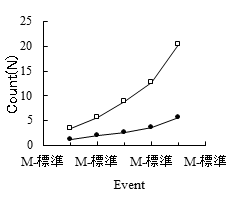
\includegraphics[keepaspectratio=true,width=0.9\linewidth,height=0.25\paperheight]{./assets/figure.png}
  \caption{The caption on a figure is put under the figure.}
  \label{fig:example figure}
\end{figure}

図表はそれらを最初に引用する文章と同じページに置くことを原則とします.
原稿末尾にまとめたりしてはいけません.
また,図表はそれぞれのページの上部または下部に集めてレイアウトして下さい.
図表の横幅は,「2段ぶち抜き」あるいはこのサンプルの
表\ref{tb:example table}や
図\ref{fig:example figure}のように
「1段の幅いっぱい」のいずれかとします.
図表の幅を1段幅以下にして図表の横に本文テキストを配置することはやめて下さい.
図表と文章本体との間には1~2行程度の空白を空けて区別を明確にします.

\subsection{図表中の文字及びキャプション}

図表中の文字や数式の大きさが小さくなり過ぎないように注意して下さい.
特にキャプションの大きさ(9pt.)より小さくならないようにして下さい.
長いキャプションは表\ref{tb:example table}のようにインデントして折り返します.

\section{参考文献の引用とリスト}

参考文献は出現順に番号を振り,その引用箇所でこのように
\cite{物部水理学:inbook}
上付き右括弧付き数字で指示します.
参考文献はその全てを原稿の末尾にまとめてリストとして示し,脚注にはしないで下さい.

\section{最終ページのレイアウトと英文要旨}

最終ページには英文のタイトル,著者名及び要旨を横1段組で書きます.
このサンプルにあるように,
本文や参考文献リストまでの2段組部分の左右の柱の高さをほぼ同じにし,
10 mm程度の空白を入れて英文要旨を配置します.
英文要旨部分の幅はタイトル部分と同じく本文よりも左右を10 mm狭くします.

  %% Bibliography
  \printbibliography[title=参考文献]
\end{multicols}
%% English Title, Author, Supervisor and Abstract
\begin{center}
  \parbox[t]{150mm}{
    \begin{center}
      \large{
        FORMATTING MANUSCRIPT. FOR ADVANCED GRADUATION RESEARCH II

        \\
        \vspace{2ex}
        Advanced Civil Engineering Jiro DOBOKU

        \\
        Supervisor: Taro SENKO

        \\
      }
    \end{center}
    \vspace{1ex}
    \small{
      \hspace*{1em}
      This template is prepared for your preparation of manuscript.
for advanced graduarion research II.
It provides instructions: page layout, font style and size and others.
If you replace the relevant text with your own by using “cut \& paste,”
you can make your manuscript.
easily.
The English ABSTRACT should be justified,
leaving a 30 mm margine on the left and right sides.
Font should be a 10-point Times-New-Roman.
The length should be 300 words or less.
It should be placed be-low the title and authors’ names set in 12 pt.,
spacing a single line.

    }
  }
\end{center}
\end{document}
